\chapter{Komunikacja}\label{ch:komunikacja}
Aby móc korzystać z robota, opracowany został protokół komunikacyjny, według którego
odbywa się komunikacja, poprzez wysyłanie jednobajtowych znaków poprzez emulowany port szeregowy. Po stronie robota Raspberry Pi wykorzystuje
sterownik \texttt{g\_serial}~\cite{g_serial}, który odopowiedzialny jest za tę emulację. Z robotem może komunikować się 
każde urządzenie z systemem Linux lub Windows. 

% \section{Komunikacja} % Bardzo możliwe że nazwa do zmiany 
Komunikacja między robotem i drugim urządzeniem odbywa się za pośrednictwem przewodu USB.
Do obsługi komunikacji wykorzystywany jest skrypt wykonany w języku Python, który jest uruchamiany 
przez \texttt{systemd}~\cite{systemd} po uruchomieniu robota. Po uruchomieniu robot czeka na komendę, która wybierze jego tryb pracy.
Obecnie do wyboru pracy osbługiwane są znaki 'e' i 'd', w przypadku otrzymania innych znaków są one ignorowane, a robot czeka aż otrzyma jeden z obsługiwanych znaków.
Po rozpoczęciu jednego z trybów pracy możliwe jest zakończenie tego trybu, wysyłając do robota znak 'q'. Sprawi to, że robot wróci do stanu, w którym czeka na wybranie 
trybu pracy. Zważywszy na to, że do wykonywania rzutów używana jest kość ośmiościenna, 
każdy rzut generuje 3 bity, tak jak zostało opisane w rozdziale~\ref{subsec:interpretacja-wyniku}.

% https://docs.kernel.org/usb/gadget_serial.html

\section{Tryb pracy} \label{sec:tryby}

\subsection{Ciągłe generowanie danych}
Aby wykorzystać ten tryb pracy, należy wysłać do robota znak 'e'.
W tym trybie zadaniem jest ciągłe generowanie kolejnych bajtów danych.
Odbywa się to przez wykonanie następującego algorytmu:
\begin{enumerate}
    \item Utowrzenie zmiennej \textit{num} i przypisanie wartości początkowej 0.
    \item Wykonanie rzutu kością.
    \item Wykorzystanie modelu opisanego w rozdziale~\ref{ch:odczytywanie-losowego-wyniku-z-kosci} do oczytania liczby i dodanie jej do zmiennej \textit{num}.
    \item Przesunięcie bitowe zmiennej \textit{num} w lewo o 3 bity, ponieważ każdy rzut generuje 3 bity.
    \item Powtórzenie kroku 1, 2 i 3 aż do wygenerowania co najmniej 8 bitów, ponieważ generując bajty, należy wykonać
    kolejno 3 rzuty (zostaje 1 bit), 3 rzuty (zostają 2 bity), 2 rzuty (wykorzystujemy bity pozostałe z poprzednich rzutów).
    \item Wydobycie bajtu ze zmiennej \textit{num}, wykonując koniunkcję binarną z liczbą 255 i wysłanie go do drugiego urządzenia.
    \item Przesunięcie bitowe zmiennej \textit{num} w prawo o 8 bitów, przez co zostanie usunięta część, która została już wysłana.
\end{enumerate}

W powyższym algorytmie dane wysyłane są po bajcie danych, ponieważ jest to najmniejsza jednostka, 
%ponieważ dane w pamięci są wyrównane do bajtów więc jest najmniejszą jednostką
którą można przekazać na raz wykorzystując \texttt{pySerial}.
Głównym założeniem tego trybu pracy jest wykorzystanie go jako dodatkowe źródło entropii w systemie 
Linux poprzez wypełnienie \textit{/dev/random}, dla zobrazowania tego wykonany został rys.~\ref{fig:interface_a}. 
Ten tryb pracy może również zostać wykorzystany w celach 
kryptograficznych na przykład w trakcie generowania kluczy.

\begin{figure}[H]
    \centering
    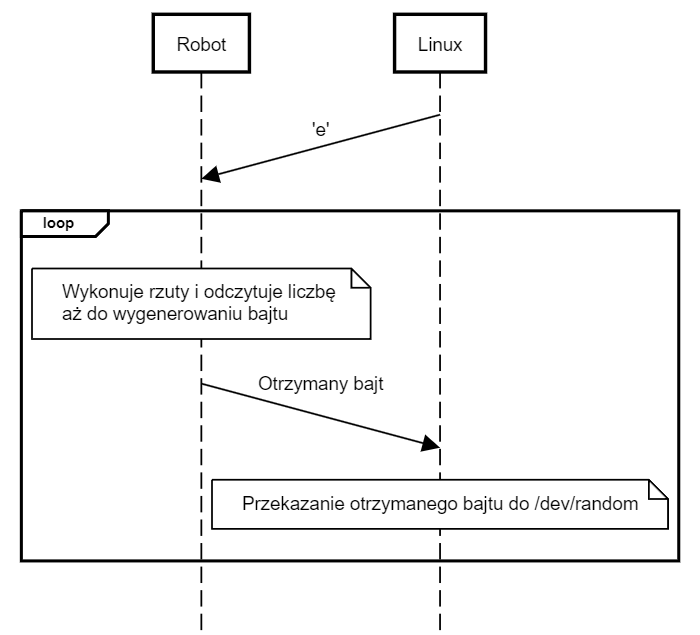
\includegraphics[width=0.5\linewidth]{chapters/05-Przetwarzanie Wyniku/figures/InterfaceA}
    \caption{Diagram sekwencji dla ciągłego generowania danych}
    \label{fig:interface_a}
\end{figure}

\subsection{Wykonywanie pojedyńczych rzutów}
Aby wykorzystać ten tryb pracy, należy wysłać do robota przez port szeregowy znak 'd'.
W tym trybie zadaniem jest oczekiwanie na polecenie wykonania rzutu, czyli znak 'r'.
Innym obsłużonym znakiem jest 'q', który spowoduje powót do wyboru trybu pracy, pozostałe znaki są ignorowane. % Robot płonie brzmi zabawniej 
Kolejnie wykonanie rzutu kością i odpowiedź otrzymaną liczbą. Następnie otrzymaną 
liczbę można wykorzystać w swoim programie. Działanie to zobrazowano na rys.~\ref{fig:interface_b}.

\begin{figure}[H]
    \centering
    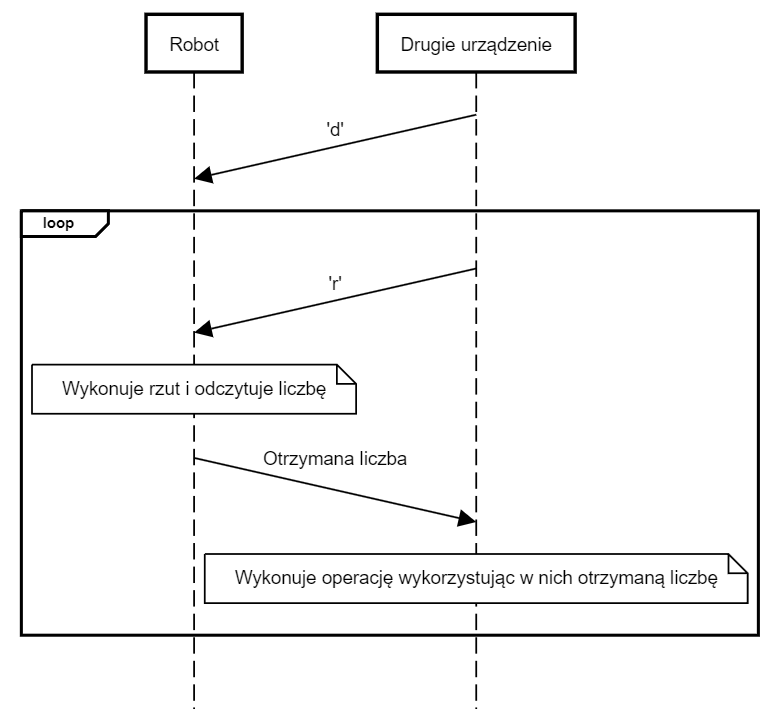
\includegraphics[width=0.5\linewidth]{chapters/05-Przetwarzanie Wyniku/figures/InterfaceB}
    \caption{Diagram sekwencji dla wykonania rzutu na żądanie}
    \label{fig:interface_b}
\end{figure}

